\chapter{Podstawy teoretyczne}

\section{Uczenie maszynowe}
\definicja{Uczenie maszynowe} (\english{Machine Learning}) to dziedzina informatyki zajmująca się konstruowaniem \textit{systemów uczących się} \cite{krawiec2003uczenie}. Podstawową cechą takich systemów jest to, że potrafią one zmieniać sposób swojego działania w miarę jak napływają do nich kolejne dane. Zmiana działania systemu może mieć różną skalę - od zmiany pojedynczych parametrów programu, przez zapamiętywanie danych wejściowych po całkowitą zmianę wykonywanego algorytmu. Niezależnie od skali każda taka zmiana powinna mieć wpływ na jego przyszłe działanie i powinna mieć na celu uzyskanie jak najwyższej \definicja{oceny} pracy systemu. Jak ujmuje to Tom Mitchell \cite{Mitchell:1997:ML:541177}:
\begin{quote}
System uczy się z doświadczenia \textit{E} ze względu na pewną klasę zadań \textit{T} i ocenę wykonania \textit{P} jeśli ocena wykonania zadań należących do klasy \textit{T} rośnie wraz z doświadczeniem \textit{E}.
\end{quote}


%Należy jednak pamiętać, że nawet najbardziej wyrafinowany system uczący ostatecznie wykonuje tylko pewną deterministyczną funkcję na danych wejściowych.  jednak proces obliczania wyniku może być rozłożony w czasie - jako dane wejściowe można traktować zarówno dane użyte do uczenia systemu, jego oceny jak i dane aktualnie do niego wprowadzane.

Systemy uczące się mają wiele zastosowań, między innymi:
\begin{itemize}
	\item Rozpoznawanie mowy ludzkiej
	\item Rozpoznawanie tekstu pisanego (\akronim{OCR}, \english{Optical Character Recognition}
	\item Diagnostyka medyczna
	\item Klasyfikacja tekstów, np. na potrzeby filtrowania niechcianych wiadomości
	\item Automatyczna identyfikacja zagrożeń na podstawie obrazu z kamer przemysłowych
	\item Kierowanie autonomicznymi pojazdami
	\item Prognozowanie pogody
	\item Prognozowanie zmian kursów akcji na giełdzie
	\item Wykrywanie podejrzanych transakcji finansowych
	\item Biometria - identyfikacja ludzi na podstawie cech takich jak głos, wygląd twarzy, odciski palców, sposób chodzenia
	\item Wspomaganie podejmowania decyzji
\end{itemize}

\subsection{Systemy klasyfikujące}
Jednym z typów systemów uczących się są \emph{systemy klasyfikujące} (inaczej \emph{klasyfikatory}). Operują one na zbiorach \emph{przykładów} opisanych za pomocą pewnego zbioru \emph{atrybutów}.
\emph{Przykłady} (zwane też \definicja{obserwacjami}) reprezentują pewne obiekty, które różnią się od siebie wartościami atrybutów. Każdy przykład jest całkowicie scharakteryzowany przez swoje wartości atrybutów, co oznacza, że dwa przykłady o identycznych wartościach atrybutów są z punktu widzenia systemu klasyfikującego nieodróżnialne. Przykładem zbioru przykładów może być np. zbiór pacjentów, zaś zbiorem atrybutów zbiór cech takich jak wiek, płeć, wzrost, wyniki testów laboratoryjnych.
Wśród zbioru atrybutów wyróżnia się jeden specjalny atrybut zwany atrybutem decyzyjnym (w odróżnieniu od pozostałych - atrybutów warunkowych) zwany też klasą lub etykietą obiektu.
Zazwyczaj wartość tego atrybutu nie jest znana bezpośrednio, jej zdobycie stanowi pewną wartość. W przytoczonym przypadku pacjentów takim atrybutem może być na przykład diagnoza choroby.
Uczenie systemu klasyfikującego polega na dostarczeniu do systemu zbioru przykładów z przypisanymi etykietami. Zbiór taki nazywamy \emph{zbiorem trenującym / uczącym}. Na podstawie przykładów ze zbioru uczącego system wytwarza wewnętrzną reprezentację, która następnie umożliwia przypisanie nieznanych klasyfikatorowi etykiet/klas nowym przykładom, które nie występowały w zbiorze uczącym.

\subsubsection{Formalizacja problemu klasyfikacji}
W celu uściślenia dalszych rozważań konieczne jest wprowadzenie notacji formalnej opisującej problem klasyfikacji \cite{krawiec2003uczenie}.
Zbiór wszystkich możliwych obiektów $ x $, których dotyczy dany problem klasyfikacji, nazywany jest dziedziną i jest oznaczany przez $ U $.
Atrybut $ a_i(x): U \mapsto V_{ai} $ to dowolna funkcja określona na dziedzinie $ U $ z przeciwdziedziną $ A_i $. Zbiór wszystkich atrybutów oznaczamy przez $ A = \{ a_1, a_2,..., a_n \} $.

Każdy przykład $ x \in X $ można opisać jako wektor w n-wymiarowej przestrzeni atrybutów $ \Omega $, czyli $ \langle a_1(x), a_2(x),...,a_n(x) \rangle $.

Problem klasyfikacji polega na znalezieniu odwzorowania, które każdemu $ x_i \in D $ (gdzie $ D $ to zbiór danych wejściowych) przypisuje jego klasę $ c_i $. W przypadku klasyfikacji binarnej $ c_i \in \{ -1, 1 \} $.

\subsubsection{Metody oceny skuteczności klasyfikacji}

W celu oceny skuteczności systemu należy za jego pomocą dokonać klasyfikacji przypadków, które nie były użyte podczas jego uczenia i których etykiety są znane (choć nie dostępne klasyfikatorowi). Wyniki klasyfikacji porównuje się z właściwymi etykietami i w ten sposób szacuje skuteczność klasyfikacji.
W tym celu można wydzielić ze zbioru przykładów specjalny podzbiór, zwany \emph{zbiorem testującym}, który jest używany do testowania a w fazie uczenia klasyfikator nie ma do niego dostępu. Czasami wydziela się też \emph{zbiór walidujący}, który jest używany w trakcie uczenia w celu optymalizacji parametrów algorytmu.
Stałego podziału zbioru przykładów na zbiór trenujący, testujący i walidujący można dokonać tylko wtedy, gdy zbiory te są wystarczająco liczne. W przeciwnym przypadku może okazać się, że nie są one wystarczająco reprezentatywne i na przykład rozkład przykładów z poszczególnych klasy jest mocno skrzywiony w którymś ze zbiorów. Aby tego uniknąć można posłużyć się metodą \emph{k-krotnej walidacji krzyżowej}. Polega ona na podzieleniu zbioru na \emph{k} podzbiorów i następnie powtarzanych \emph{k}-razy fazach uczenia i testowania klasyfikatora, przy czym za każdym razem k-ty podzbiór służy jako zbiór testujący/walidujący a pozostałem podzbiory jak zbiór uczący. Skuteczności klasyfikacji oblicza się wtedy jako średnią sprawność osiąganą we wszystkich k testach.

\subsection{Miary skuteczności klasyfikacji}\label{sec:measures}
	Do oceny jakości klasyfikacji można używać różnych miar. W przypadku klasyfikacji binarnej (czyli kiedy rozróżniamy tylko dwie klasy przykładów) większość z nich można wyrazić za pomocą stosunku kilku z czterech wartości wyrażających liczbę przypadków klasyfikowanych w określony sposób. Wartości te są odnoszą się zawsze do jednej z klas, która jest w pewien sposób wyróżniona. Na przykład w przypadku diagnozy medycznej zazwyczaj taką klasą jest grupa osób chorych na jakąś chorobę. Przypadki zaklasyfikowane jako należące do tej klasy określane są jako zaklasyfikowane \textit{pozytywnie} (\english{positive}) natomiast przypadki zaklasyfikowane jako do niej nienależące jako zaklasyfikowane negatywnie (\english{negative}). Słowa \english{"True"} oraz \english{"False"} odnoszą się odpowiednio do przypadków zaklasyfikowanych prawidłowo i nieprawidłowo:
	\begin{itemize}
		\item \definicja{\textbf{True Positive (\akronim{TP})}} - liczba przypadków \textbf{poprawnie} zaklasyfikowanych jako \textbf{należące} do wyróżnionej klasy,
		\item  \definicja{\textbf{True Negative (\akronim{TN})}} - liczba przypadków \textbf{poprawnie} zaklasyfikowanych jako \textbf{nienależące} do wyróżnionej klasy,
		\item \definicja{\textbf{False Positive (\akronim{FP})}} - liczba przypadków \textbf{niepoprawnie} zaklasyfikowanych jako \textbf{należące} do wyróżnionej klasy (inaczej błąd pierwszego rodzaju)
		\item \definicja{\textbf{False Negative (\akronim{FN})}} - liczba przypadków \textbf{niepoprawnie} zaklasyfikowanych jako \textbf{nienależące} do wyróżnionej klasy (inaczej błąd drugiego rodzaju)
	\end{itemize}		
	
	 Poniżej zostały opisane miary, o których będzie mowa w dalszej części pracy. Wszystkie one zawierają się w przedziale $ \langle 0,1 \rangle $.

	\begin{itemize}
		\item \definicja{Precyzja (\english{precision})} - określa jaka część przypadków zaklasyfikowanych jako należące do wyróżnionej klasy rzeczywiście do niej należy. Dana jest wzorem:
		 $$ precision = \frac{TP}{TP+FP} $$
		
		\item \definicja{Kompletność (\english{recall})} - określa jaka część przypadków należących do wyróżnionej klasy została prawidłowo zaklasyfikowana jako należące do niej. Dana jest wzorem:
		$$ recall = {TP}{TP+FN} $$

		\item \definicja{Trafność (lub dokładność)} (\english{Accuracy}) - stosunek liczby przypadków ze zbioru walidującego, które zostały zaklasyfikowane poprawnie do liczby wszystkich przepadków w zbiorze testującym. Może być wyrażona jako:
		$$ accuracy = \frac{TP+TN}{TP+TN+FP+FN} $$

		\item \definicja{Miara $ F_{1} $ } (\english{ $ F_{1} $ measure }) - 	miara uwzględniająca zarówno precyzję (\english{precision}) jak i \definicja{kompletność} (\english{recall}). Miara ta nie uwzględnia wartości \emph{TN}. Jej wartość jest dana wzorem:
		$$ F_{1} = 2 \times \frac{precision \times recall}{precision + recall} $$
		 
		
		\item \definicja{ \akronim{MCC} \english{Matthews correlation coefficient}} - miara, która w przeciwieństwie do miary $ F_{1} $ bierze pod uwagę wszystkie cztery wartości (\emph{TP}, \emph{TN}, \emph{FP} i \emph{FN}). Dana wzorem: 
		$$ MCC = \frac{ TP \times TN - FP \times FN } {\sqrt{ (TP + FP) ( TP + FN ) ( TN + FP ) ( TN + FN ) } } $$
		
		\item \definicja{ Średnie prawdopodobieństwo wyboru właściwej klasy } - niektóre klasyfikatory zamiast przypisywać każdemu z przykładów jedną z klas potrafią zwrócić dla każdego przykładu rozkład przynależności do wszystkich rozważanych klas. Jakość klasyfikacji można wtedy obliczyć jako uśrednioną po wszystkich przykładach wartość prawdopodobieństwa przypisanego klasie, do której przykład należy. Wartość taka może wahać się od wartości 0 (kiedy dla każdego przykładu do jego właściwej klasy zostało przypisane prawdopodobieństwo 0) do wartości 1 (kiedy dla każdego przykładu do jego właściwej klasy zostało przypisane prawdopodobieństwo 1).

	\end{itemize}		

	W przypadku problemów, w których wyróżnia się $ k>2 $ klas miara korzystająca z wartości  \emph{TP},\emph{TN},\emph{FP} i \emph{FN} jest obliczana jako średnia wartość tej miary dla $ k $ problemów binarnych polegających na zaklasyfikowaniu przykładów jako należących lub nienależących do wybranej klasy.


\subsection{SVM}
    
\definicja{Maszyna wektorów wspierających } (\akronim{SVM}, \english{Support Vector Machine}) to rodzaj klasyfikatora binarnego. Stanowi on rozszerzenie \emph{klasyfikatora liniowego}, lecz w przeciwieństwie do niego jest w stanie poprawnie klasyfikować dane \emph{nieseparowalne liniowo}. Jest to możliwe dzięki dokonywanej przez SVM transformacji danych do wyższych wymiarów za pomocą \emph{funkcji jądrowych}.

\subsubsection{Klasyfikator liniowy}
Jednym z najprostszych klasyfikatorów jest \definicja{klasyfikator liniowy}. Rozwiązuje on problem klasyfikacji binarnej poprzez znalezienie w przestrzeni atrybutów $ \Omega $ hiperpłaszczyzny, która dzieli ją na dwie części odpowiadające dwóm klasom decyzyjnym: $ \{-1, 1 \} $.
\begin{definicjaa}
Hiperpłaszczyzna w przestrzeni $ \Omega $ to zbiór:
\begin{equation}
\left\{ x \in \Omega | \langle w, x\rangle + b = 0 \right\}, w \in \Omega, b \in R
\label{eq:hiperplane}
\end{equation}
$ \langle x, y \rangle $ oznacza iloczyn skalarny wektorów $ x $ i $ y $:
$$ \langle x, y \rangle = \sum_{i=1}^{N} [x]_i [y]_i $$
gdzie $ [x]_i $ to i-ta wartość wektora $ x $.
\end{definicjaa}

Wektor $ w $ we wzorze \ref{eq:hiperplane} to wektor wag, normalny do hiperpłaszczyzny, $ ||w|| $ to norma euklidesowa tego wektora, czyli jego długość, a $ b/||w|| $ to odległość płaszczyzny od początku układu współrzędnych.
Oba te parametry można razem dowolnie przeskalowywać, to jest pomnożyć $ w $ i $ b $ przez tę samą stałą zachowując tę samą hiperpłaszczyznę. Dlatego wprowadza się ograniczenie, po którego zastosowaniu otrzymujemy tak zwaną postać kanoniczną hiperpłaszczyzny:
\begin{definicjaa}
Dla danego zbioru obserwacji $ x_1, x_2, ..., x_m \in \Omega $ wektor $ w $ i parametr $ b $ wyznaczają \textbf{kanoniczną postać hiperpłaszczyzny} jeśli:
\begin{equation}
	\min_{i=1..m} | \langle w, x_i \rangle + b | = 1
\label{eq:canonical}
\end{equation}
\end{definicjaa}


Hiperpłaszczyzna dana wzorem \ref{eq:hiperplane} definiuje funkcję decyzyjną, która każdemu przypadkowi z $ \Omega $ przypisuje klasę decyzyjną:
\begin{equation}
\begin{array}{lcl}
f_{w,b}: \Omega \rightarrow \{\pm 1\} \\ x \mapsto f_{w,b}(x) = sgn (\langle w, x \rangle + b)
\end{array}
\label{eq:decfunc}
\end{equation}

\begin{figure}[h]
\centering
\includegraphics[scale=0.5]{figures/functions/2-different-hyperplanes}
\label{fig:hyperplanes}
\caption{Hiperpłaszczyzny separujące dwa zbiory punktów w przestrzeni dwówymiarowej. Każda z z nich poprawnie separuje punkty ze zbioru uczącego - zielone koła i niebieskie kwadraty. Przykłady ze zbioru testowego (puste kwadraty i kółka) są poprawnie separowane jedynie przez dwie proste (prosta narysowana linią ciągłą i prosta narysowana kropkami i keskami).}
\end{figure}

Wynikiem uczenia klasyfikatora liniowego jest znalezienie hiperpłaszczyzny i odpowiadającej jej funkcji decyzyjnej, która przykładom ze zbioru uczącego $ (x_i, y_i) \in \Omega $ przypisuje prawidłowe etykiety, czyli dla każdego (jeśli zbiór jest liniowo separowalny), lub dla jak największej liczby przypadków $ x_i $ zachodzi  $ f_w,b(x_i) = y_i $. Zazwyczaj kilka hiperpłaszczyzn równie dobrze rozdziela przypadki ze zbioru uczącego, mogą się jednak one różnić zdolnością do klasyfikacji zbioru testowego, co pokazano na rysunku \ref{fig:hyperplanes}. Optymalna hiperpłaszczyzna separująca to taka, która charakteryzuje się największym marginesem, czyli odległością hiperpłaszczyzny do najbliżej położonych obserwacji \cite{scholkopf_learning_2002}.
\begin{definicjaa} Dla hiperpłaszczyzny danej wzorem $ { x \in \Omega | \langle w, x \rangle + b = 0} $ oraz zbioru obserwacji $ {(x_1, y_1), (x_2, y_2), ..., (x_m, y_m)} $ marginesem tego zbioru od hiperpłaszczyzny nazywamy minimalną odległość hiperpłaszczyzny od punktów z tego zbioru:
	\begin{equation}
	\rho_{w,b} := \min_{i=1..m} y \times (\langle w, x \rangle + b) / ||w||
	\label{eq:margin}
	\end{equation}
	
\end{definicjaa}
Żeby maksymalizować margines powinniśmy minimalizować $ ||w|| $, zachowując warunek \ref{eq:canonical}. Problem znalezienia optymalnej hiperpłaszczyzny separującej zbiór przykładów  $ {(x_1, y_1), (x_2, y_2), ..., (x_m, y_m)} $ można zatem zapisać jako problem optymalizacyjny:
\begin{equation}
\begin{array}{lll}
\min\limits_{w \in \Omega, b \in \Re} &  \tau(w) = \frac{1}{2}||w||^2 & \\
\text{p.o.} &  y_i  (\langle w, x \rangle + b) \geq 1 & \text{ dla } i=1..m
\end{array}
\label{eq:primal}
\end{equation}
Ograniczenia w powyższym problemie zapewniają, że wartość funkcji decyzyjnej $ f_{w,b}(x_i) $ będzie równa $  y_i $, czyli, że hiperpłaszczyzna poprawnie odseparuje przykłady z dwóch grup. Osiągnięcie celu optymalizacji zapewnia znalezienie hiperpłaszczyzny o maksymalnym marginesie.

\begin{figure}[h]
\centering
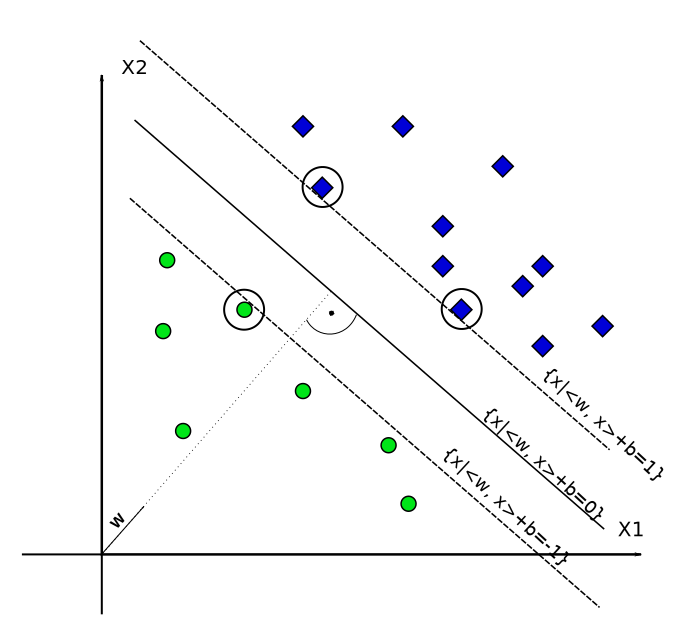
\includegraphics[scale=0.5]{figures/functions/2-margin}
\label{fig:margin}
\caption{Hiperpłaszczyzna separująca dwa zbiory punktów w przestrzeni dwuwymiarowej wraz z marginesami. Przykłady w kółku to wektory podpierające.}
\end{figure}


Powyższy problem programowania matematycznego jest podany w tak zwanej \definicja{formie prymalnej}. W praktyce rozwiązuje się wersję \definicja{dualną} problemu, która ma przyjmuje następującą postać:

\begin{definicjaa} Wersja dualna problemu znalezienia optymalnej hiperpłaszczyzny:
\begin{equation}
\begin{array}{ll}
\max\limits_{\alpha \in R^m} & W(\alpha) = \sum_{i=1}^{m} \alpha_i - \sum_{i,j=1}^{m} \alpha_i \alpha_j y_i y_j \dotp{x_i}{x_j} \\
\text{p.o.} &  \alpha_i \geq 0 , \text{ dla } i=1..m \\
& \sum_{i=1}^{m} \alpha_i y_i = 0
\end{array}
\label{eq:dual}
\end{equation}
%\begin{align}
%\max_{\alpha \in R^m} &\qquad  W(\alpha) = \sum_{i=1}^{m} \alpha_i - \sum_{i,j=1}^{m} \alpha_i \alpha_j y_i y_j \dotp{x_i}{x_j} \\
%p.o. &\qquad {}  \alpha_i \geq 0 , dla i=1..m \\
%&\qquad {} \sum_{i=1}^{m} \alpha_i y_i = 0 	
%\end{align}
\end{definicjaa}

Dla formy dualnej problemu optymalizacji funkcja decyzyjna przyjmuje postać:
\begin{equation}
f(x) = sgn \left( \sum_{i=1}^{m} y_i a_i \dotp{x}{x_i} + b \right)
\end{equation}

W przypadku, w którym dane nie są separowalne liniowo, tzn. nie istnieje taka hiperpłaszczyzna, która dla danego zbioru przykładów spełnia ograniczenia ze wzoru \ref{eq:primal}, do problemu optymalizacyjnego wprowadza się tak zwane \definicja{zmienne osłabiające} (\english{slack variables}) $ \zeta_i, i=1..m $.
Wzór \ref{eq:primal} przyjmuje wówczas postać: 

\begin{equation}
\begin{array}{lll}
\min\limits_{w \in \Omega, b \in \Re} &  \tau(w) = \frac{1}{2}||w||^2 + \frac{C}{m} \sum_{i=1}^{m} \zeta_i & \\
\text{p.o.} &  y_i  (\langle w, x \rangle + b) \geq 1 - \zeta_i & \text{ dla } i=1..m \\
& \zeta_i \geq 0 & \text{ dla } i=1..m \\
\end{array}
\label{eq:primal-c}
\end{equation}

Natomiast wzór \ref{eq:dual}:
\begin{equation}
\begin{array}{ll}
\max\limits_{\alpha \in R^m} & W(\alpha) = \sum_{i=1}^{m} \alpha_i - \sum_{i,j=1}^{m} \alpha_i \alpha_j y_i y_j \dotp{x_i}{x_j} \\
\text{p.o.} & 0 \leq \alpha_i \leq \frac{C}{m} , \text{ dla } i=1..m \\
& \sum_{i=1}^{m} \alpha_i y_i = 0
\end{array}
\label{eq:dual-c}
\end{equation}

\definicja{Wektory wspierające}

\subsubsection{Maszyny wektorów wspierających}

\begin{itemize}
\item \definicja{Transformacja}
\item \definicja{Kernel Trick}
\end{itemize}

\section{Obliczenia ewolucyjne}

Obliczenia ewolucyjne to ...

\begin{itemize}
\item \definicja{osobnik}
\item \definicja{populacja}
\item \definicja{pokolenie}
\item \definicja{mutacja}
\item \definicja{krzyżowanie}
\item \definicja{selekcja}
\item \definicja{funkcja przystosowania} (\english{fitness})
\end{itemize}

\subsection{Programowanie genetyczne}
\definicja{Programowanie genetyczne} (\akronim{GP}, \english{Genetic Programming}) to 

Funkcje, które generuje algorytm programowania genetycznego są w nim reprezentowane w postaci drzew. Węzłami takiego drzewa są elementarne funkcje zadeklarowane w kodzie programu. Każda z takich funkcji ma przypisane pewne ograniczenia co do ilości i typu argumentów, które przyjmuje oraz co do typu wartości, który zwraca. Drzewo jako całość również ma zadeklarowany typ zwracanej wartości.

\section{Ewolucja kerneli}

%\section{Obrazowanie mózgu przy pomocy rezonansu magnetycznego}
%\begin{itemize}
%\item \definicja{Obrazowanie metodą rezonansu magnetycznego} (\akronim{MRI}, \english{Magnetic Resonance Imaging})
%\item \definicja{Obrazowanie metodą funkcjonalnego rezonansu magnetycznego} (\akronim{fMRI}, \english{functional Magnetic Resonance Imaging})
%\end{itemize}
\clearpage